\vspace{1cm}

Two charts have been given below which show the various mission concepts that are possible in all the fields that have been mentioned above along with the science requirements that are required for each of these missions. 
\begin{figure}[!ht]
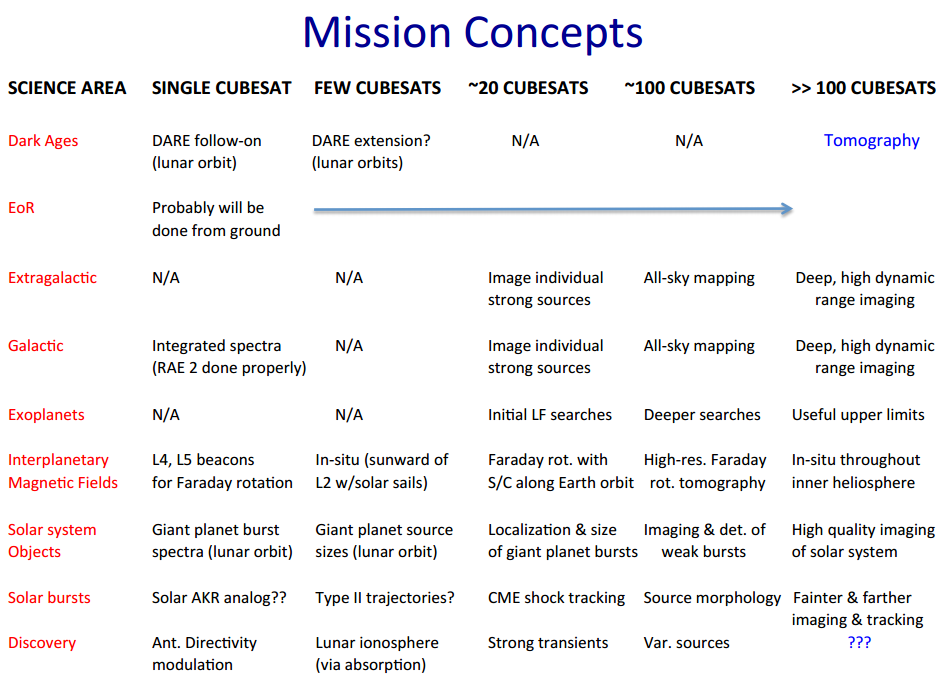
\includegraphics[scale=0.7]{mission_concepts.png}
\caption{Mission concepts for multiple agent systems in all fields (source: \href{http://kiss.caltech.edu/workshops/smallsat2012/presentations/low_freq_missions.pdf}{Presentation by Dayton Jones})}
\end{figure}

\begin{figure}[!ht]
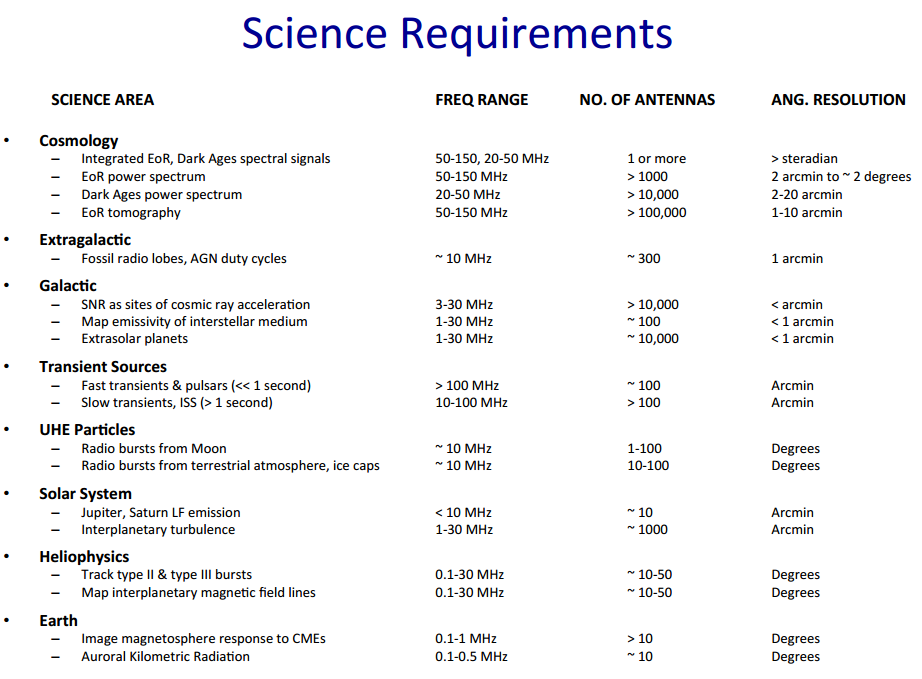
\includegraphics[scale=0.7]{science_req.png}
\caption{Science Requirements for above missions(source: \href{http://kiss.caltech.edu/cosponsored/cubesat2012/presentations/low_freq_science_req.pdf}{Presentation by Dayton Jones})}
\end{figure}
\newpage

\vspace{1cm}
All the missions that have been mentioned above have been plotted on graph as shown below. The vertical axis has the number of satellites that are required to perform that particular mission. The horizontal axis has been split according to whether it can be performed using a single spacecraft or whether formation flying or constellations are required to do the same. They have been colour coded according to the mission class and bigger the size, the costlier the mission. 

\begin{figure}[!ht]
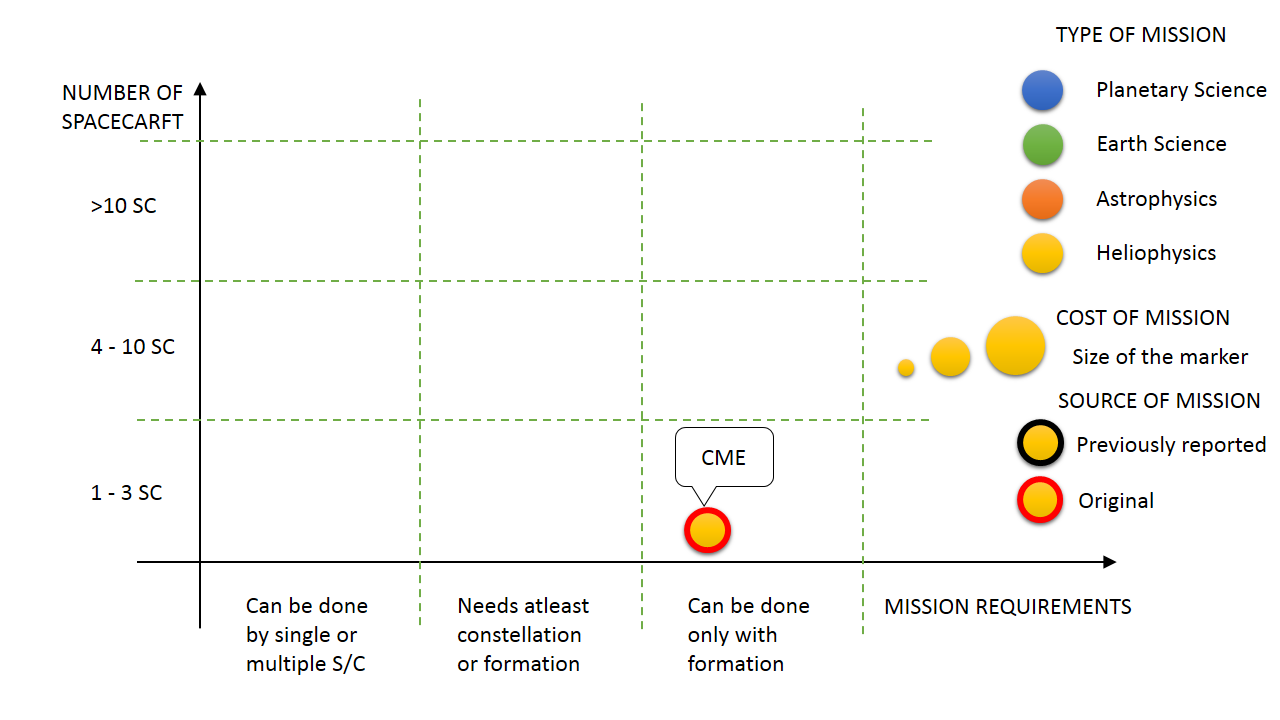
\includegraphics[scale=0.5]{cost_function.png}
\caption{Mission Categorization}
\end{figure}
\newpage
%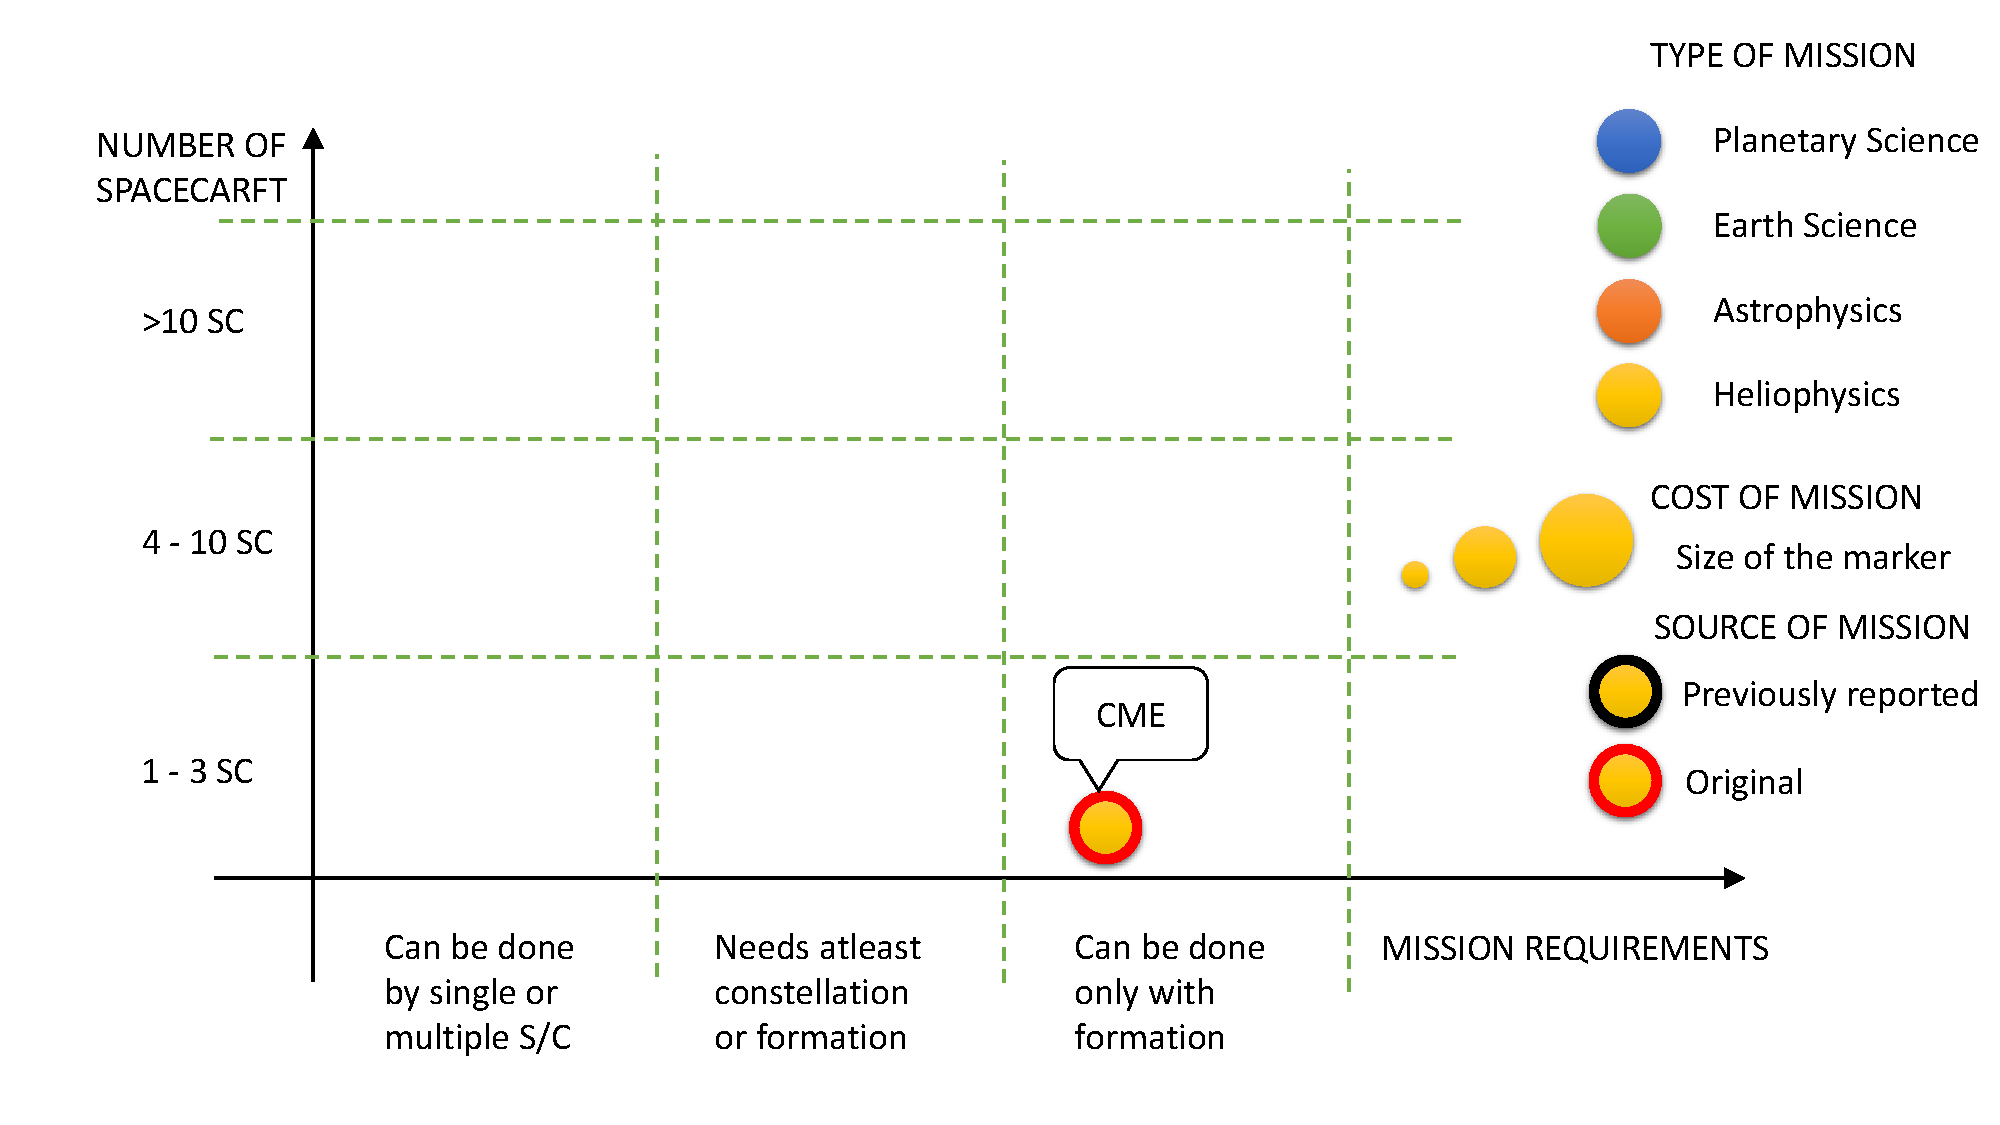
\includepdf[scale = 0.5]{cost_function.pdf}